% Перестроение в двумерном случае.
\subsection{Методы перестроения поверхности в двумерном случае}

Рассмотрим геометрическую задачу о перестроении поверхности в двумерном пространстве в общем виде \cite{Rybakov2019Geo2D}.
Пусть даны $n$ ячеек поверхностной сетки, каждая из которых представлена отрезком длины $l_i$ (то есть общее количество узлов равно $n + 1$).
Известно направление изменения поверхности каждой ячейки (направление нормали к отрезку), а также направление движения каждого узла $\overline{g_i}$, $|\overline{g_i}| = 1$.
Оно совпадает с направлением суммы единичных нормалей, проведенных к инцидентным ячейкам.
К тому же для двумерного случая это направление лежит на биссектрисе угла, образованного двумя инцидентными ячейками \cite{Fortin2004Remesh2d} (рис.~\ref{fig:text_1_remesh_2d_grid_normals}).

\begin{figure}[h]
\onelinecaptionstrue
\centering
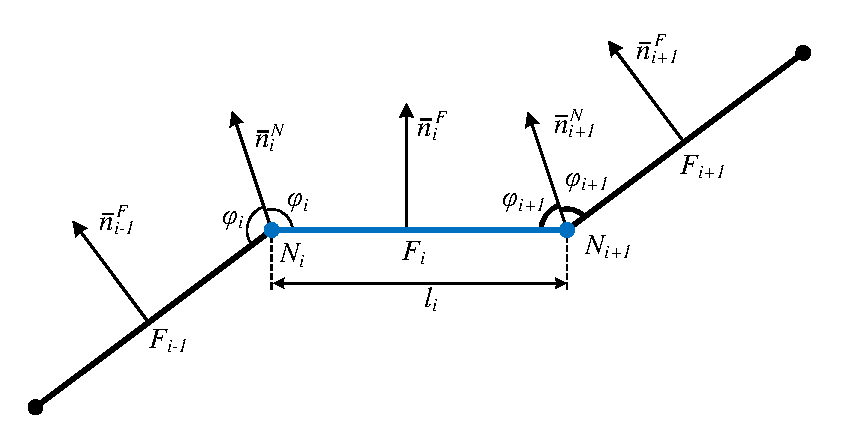
\includegraphics[width=0.7\textwidth]{pics/text_1_remesh_2d/grid_normals.pdf}
\captionstyle{normal}\caption{Поверхностная сетка с обозначенными направлениями движения узлов.}
\label{fig:text_1_remesh_2d_grid_normals}
\end{figure}

Также известны локальные сдвиги поверхности для каждой ячейки (они задаются значениями $H_i$).
Требуется найти такие значения локальных сдвигов узлов сетки $h_i$, чтобы охватывающая площадь между исходной поверхностью и новой поверхностью для каждой ячейки сетки ($S_i$) как можно меньше отличалась от требуемого значения $T_i = l_iH_i$.

Для решения данной задачи сначала требуется вычислить охватываемую площадь для каждой отдельной ячейки.

\subsubsection{Задача о вычислении охватываемой площади при движении узлов отдельной ячейки}

Рассматривается ячейка, представленная на плоскости отрезком $AB$ длины $l$.
При перемещении точек $A$ и $B$ в новые точки $A_1$ и $B_1$ соответственно образуется четырехугольник $AA_1B_1B$.
Требуется найти его площадь, выраженную явно через параметры $a = \overline{AA_1}$ и $b = \overline{BB_1}$ (рис.~\ref{fig:text_1_remesh_2d_local}).

\begin{figure}[h]
\onelinecaptionstrue
\centering
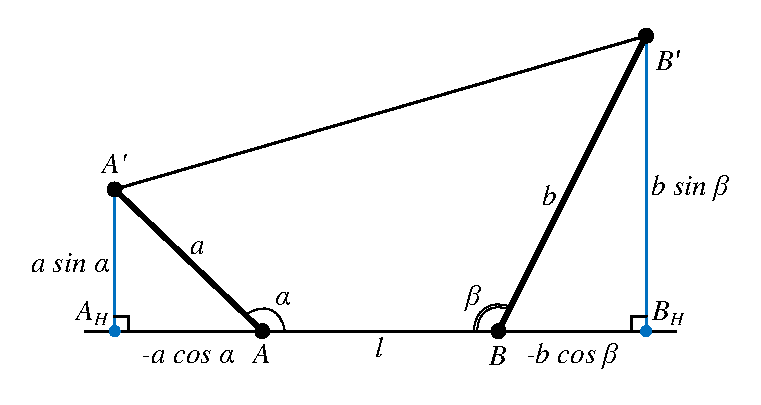
\includegraphics[width=0.7\textwidth]{pics/text_1_remesh_2d/local.pdf}
\captionstyle{normal}\caption{Вычисление охватываемой площади при передвижении узлов ячейки.}
\label{fig:text_1_remesh_2d_local}
\end{figure}

Для решения задачи опустим перпендикуляры из точек $A_1$ и $B_1$ на прямую $AB$.
Их основаниями будут точки $A_2$ и $B_2$ соответственно.
Искомая площадь может быть представлена в следующем виде:
\begin{equation}
S_{AA_1B_1B} = S_{A_2A_1B_1B_2} - S_{AA_1A_2} - S_{BB_1B_2}
\end{equation}

Обозначим угол между векторами $\overline{AA_1}$ и $\overline{AB}$ через $\alpha$, а угол между векторами $\overline{BB_1}$ и $\overline{BA}$ через $\beta$.
Тогда искомая площадь вычисляется явно в следующем виде:
\begin{equation}
S_{AA_1B_1B} = \frac{1}{2}(l - a \cos \alpha - b \cos \beta)(a \sin \alpha + b \sin \beta) + \frac{1}{2}a^2 \sin \alpha \cos \alpha + \frac{1}{2}b^2 \sin \beta \cos \beta
\end{equation}

\begin{equation}
S_{AA_1B_1B} = \frac{1}{2}\big(l(a \sin \alpha + b \sin \beta) - ab \sin(\alpha + \beta)\big)
\end{equation}

\subsubsection{Поиск смещений узлов методом градиентного спуска}

Метод градиентного спуска является одним из наиболее простых методом оптимизации для нахождения локального минимума функции.
При условии, что в любой точки функции можно вычислить ее градиент, то начиная с некоторого начального приближения $x_0$ строится итерационная последовательность~\cite{Kantorovich1984Func}:
\begin{equation}
x^{k+1} = x^k - \gamma_k \nabla f(x_k)
\end{equation}

где $\gamma_k \ge 0$ задает длину шага и, соответственно, скорость градиентного спуска.

Градиентный метод находит свое основное применение в задаче поиска минимума или максимума функции.
Направление антиградиента является направлением наискорейшего убывания функции.
Основная проблема метода заключается в выборе шага $\gamma$.
При слишком больших значениях шага существует вероятность миновать искомый минимум функции.
К тому же, метод не гарантирует нахождение глобального минимума.

Рассмотрим решение поставленной задачи методом градиентного спуска.
Неизвестными параметрами являются величины сдвигов узлов сетки $h_i$ для $0 \le i \le n$.
Опираясь на решение локальной задачи об определении охватываемой площади, можно записать охватываемую площадь при движении отдельной ячейки:
\begin{equation}
S_i = \frac{1}{2}\big(l_i(h_i \sin \alpha_i + h_{i + 1} \sin \beta_i) - h_ih_{i + 1} \sin(\alpha_i + \beta_i)\big) 
\end{equation}

Отклонением охватываемой площади в ячейке от истинного значения будем называть величину $\delta_i = S_i - T_i$, а ошибкой -- ее квадрат $d_i = \delta_i^2$.
Общая ошибка при перестроении поверхности задается как сумма ошибок для всех ячеек:
\begin{equation}
D = \sum_{i = 0}^{n - 1}{d_i}
\end{equation}

При нахождении оптимального решения требуется минимизировать общую ошибку.
Для нахождения градиента требуется вычислить частные производные функции $D$ по всем неизвестным $h_i$.
Эти частные производные можно записать в явном виде:
\begin{equation}
\frac{\partial D}{\partial h_i} = \frac{\partial d_{i - 1}}{\partial h_i} + \frac{\partial d_i}{\partial h_i}
\end{equation}

где
\begin{equation}
\begin{cases}
\frac{\partial d_{i - 1}}{\partial h_i} = \delta_{i - 1}(l_{i - 1} \sin \beta_{i - 1} - h_{i - 1} \sin(\alpha_{i - 1} + \beta_{i - 1})) \\
\frac{\partial d_i}{\partial h_i} = \delta_i(l_i \sin \alpha_i - h_{i + 1} \sin(\alpha_i + \beta_i))
\end{cases}
\end{equation}

\

Также при осуществлении метода градиентного спуска требуется следить за соблюдением дополнительных условий, которые накладываются на неизвестные $h_i$.
Например, очевидным условием является выполнение соотношения $h_i \ge 0$, что запрещает движение сетки в отрицательном направлении.
В нашем случае использовались более строгие условия $\min(H_{i - 1}, H_i) \le h_i \le \max(H_{i - 1}, H_i)$, которые не позволят величинам смещения узлов сетки выходить за пределы смещений инцидентных им ячеек сетки.

\subsubsection{Приближенные методы перестроения поверхности}

Решение задачи о перестроении сетки методом градиентного спуска оказывается слишком требовательной к ресурсам задачей при увеличении размера сетки.
К тому же качество решения зачастую оказывается неудовлетворительным, особенно при попадании в локальные минимумы.
Поэтому для решения поставленной задачи рассмотрим методы приближенного решения, основанные на аппроксимации решения в каждой ячейке с помощью примитивных геометрических фигур.

В качестве первого метода рассмотрим приближение, при котором каждый узел сетки сдвигается на вектор $\frac{1}{2}(H_{i - 1} + H_i)\overline{g_i}$.
Этот метод соответствует приближению решения в каждой ячейке прямоугольником по сторонами $l_i$ и $H_i$, а затем усреднения, как показано на рис.~\ref{fig:text_1_remesh_2d_grid_rectangles}.

\begin{figure}[h]
\onelinecaptionstrue
\centering
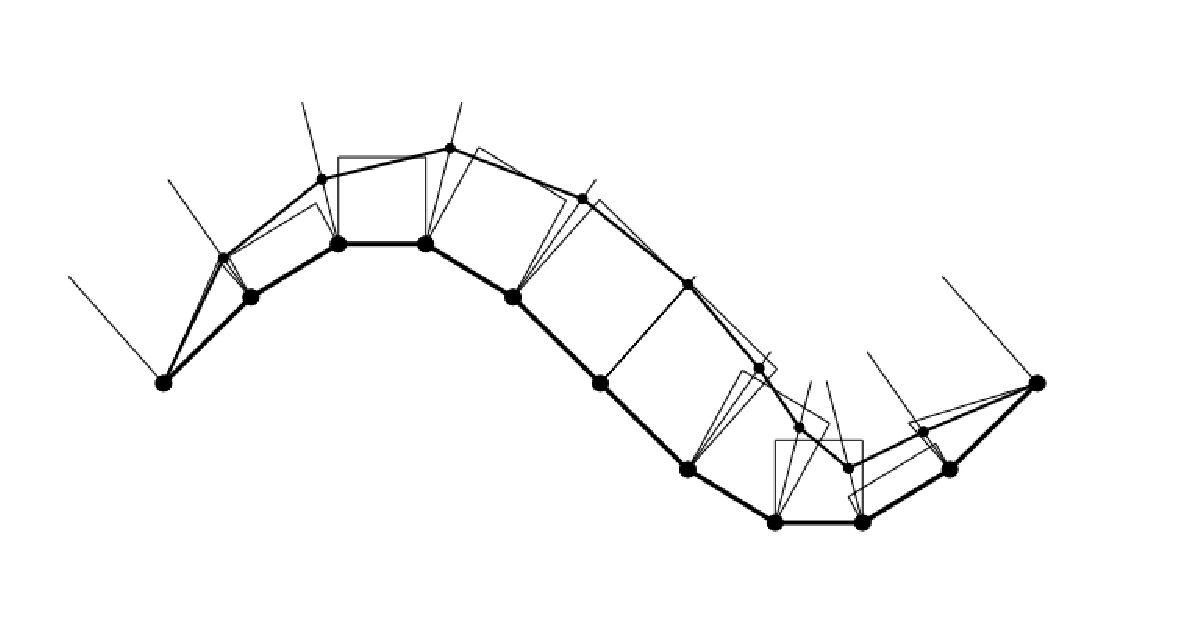
\includegraphics[width=0.7\textwidth]{pics/text_1_remesh_2d/grid_rectangles.pdf}
\captionstyle{normal}\caption{Перестроение поверхности методом прямоугольников.}
\label{fig:text_1_remesh_2d_grid_rectangles}
\end{figure}

В методе трапеций решение в каждой ячейке приближается трапецией с площадью $T_i$, боковые стороны которой лежат на направлениях роста двух узлов, относящихся к рассматриваемой ячейке.
После построения трапеций для всех ячеек сетки у каждого внутреннего узла появляется две новые потенциальные позиции для сдвига (образованные ячейкой слева и ячейкой справа).
В качестве финальной новой позиции выбирается их среднее значение (рис.~\ref{fig:text_1_remesh_2d_grid_trapeziums}).

\begin{figure}[h]
\onelinecaptionstrue
\centering
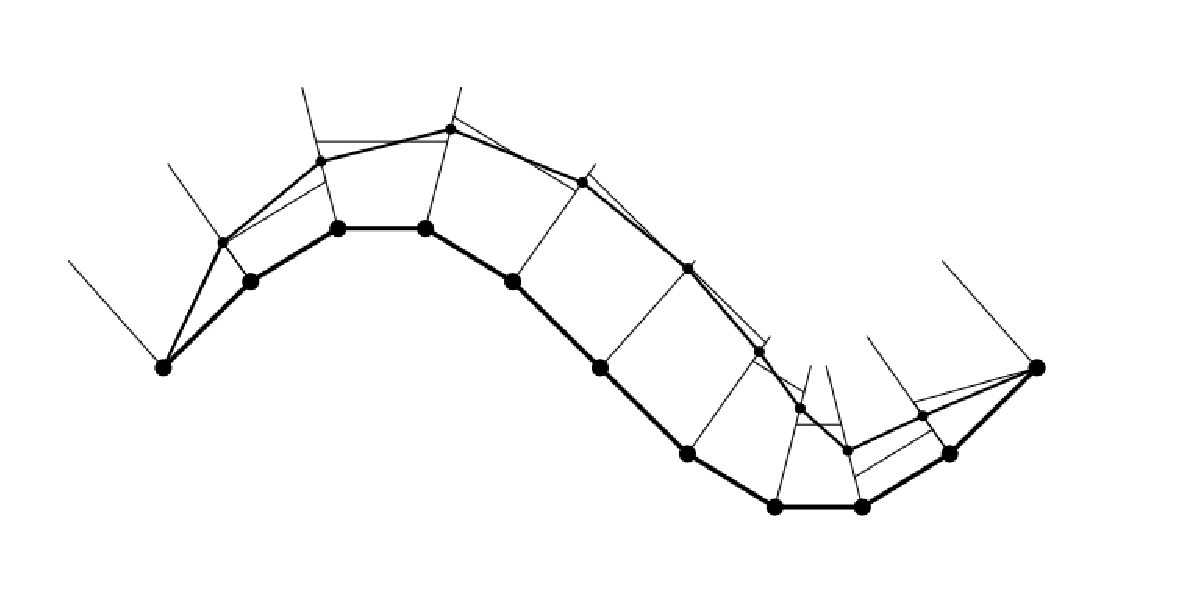
\includegraphics[width=0.7\textwidth]{pics/text_1_remesh_2d/grid_trapeziums.pdf}
\captionstyle{normal}\caption{Перестроение поверхности методом трапеций.}
\label{fig:text_1_remesh_2d_grid_trapeziums}
\end{figure}

Для сравнения точности решений, полученных с помощью описанных методов была использована модельная двумерная поверхностная сетка, представленная одним периодом синусоиды ($x \in [0, 2 \pi]$).
В качестве набора смещений ячеек ($H_i$) использовались одинаковые смещения на величину, равную половине размера ячейки.
При увеличении количества узлов оба приближенных метода продемонстрировали стремление к нулю величины $\frac{D}{\sum_i{T_i}}$ с незначительными отклонениями друг от друга и от метода градиентного спуска, который использовался для верификации.
Также было проведено сравнение величин $\delta_i$ для всех ячеек для рассмотренных приближенных методов.
Результаты сравнения на модельной сетке при количестве узлов $n = 1000$ приведены на рис.~\ref{fig:text_1_remesh_2d_graphic}.

\begin{figure}[h]
\onelinecaptionstrue
\centering
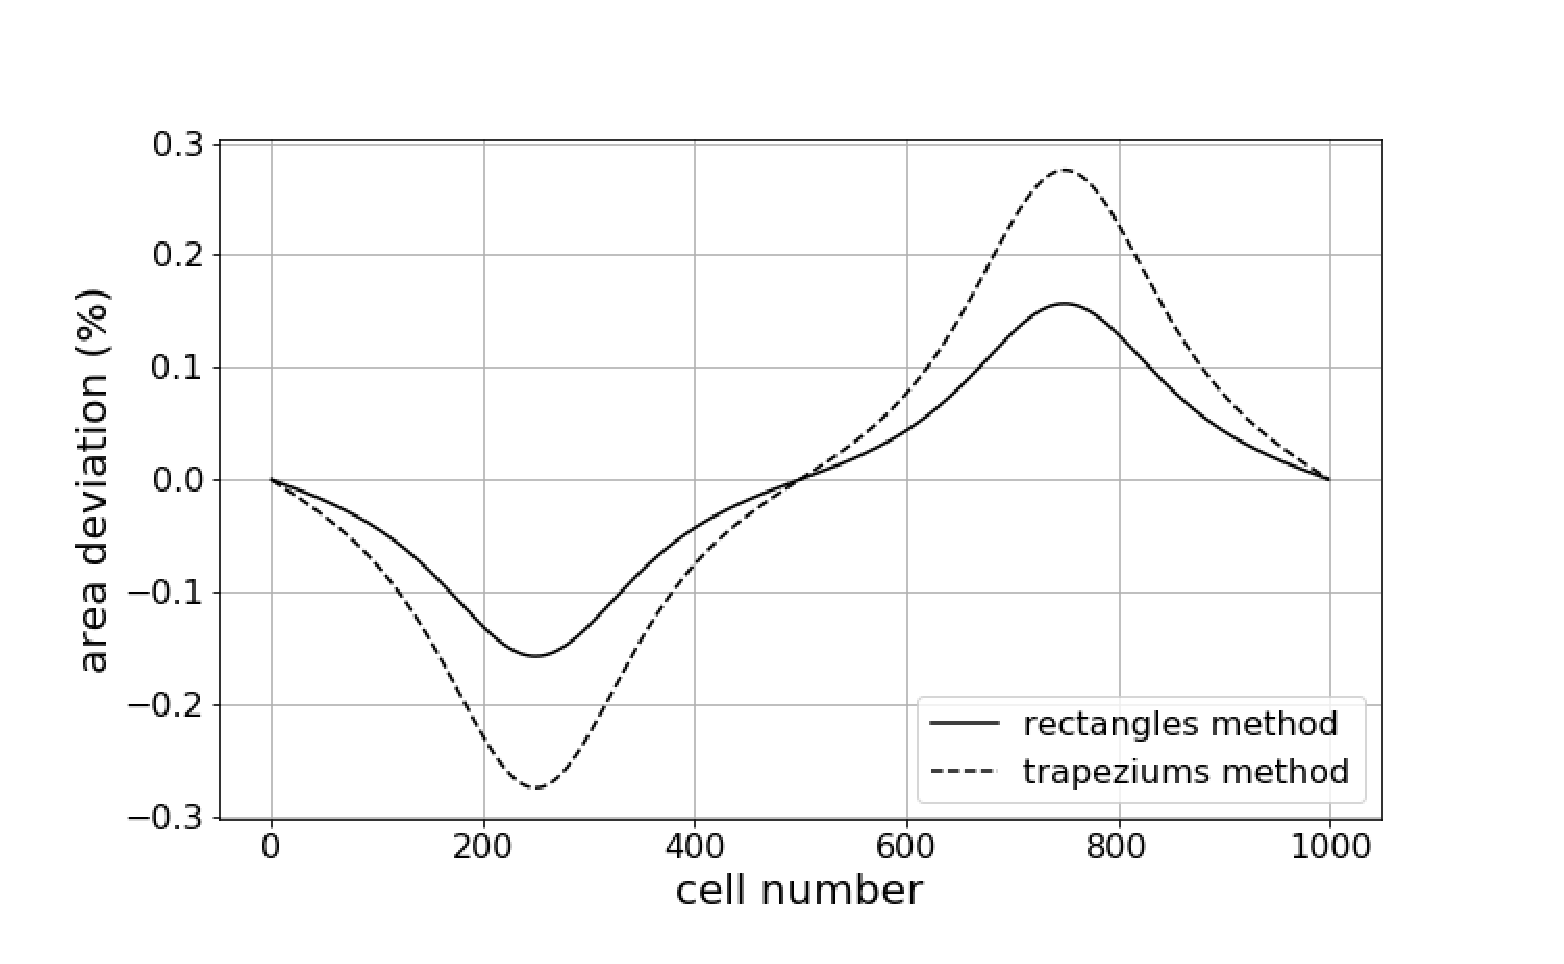
\includegraphics[width=0.8\textwidth]{pics/text_1_remesh_2d/graphic.pdf}
\captionstyle{normal}\caption{Сравнение точности решений методом прямоугольников и методом трапеций.}
\label{fig:text_1_remesh_2d_graphic}
\end{figure}

Из графика на рис.~\ref{fig:text_1_remesh_2d_graphic} видно, что более простой метод прямоугольников является в то же время и более точным, так как обеспечивает меньшие отклонения от точного решения на сильно выпуклых и сильно вогнутых участках сетки.

В заключение приведем теоретическую оценку точности приведенных методов перестроения поверхности.
Оценку будем производить для модельной расчетной сетки, которая удовлетворяет следующим требованиям.
Все ячейки сетки одинаковые и имеют длину $l$, смещения всех ячеек одинаково и равно $H$, кривизна сетки (угол отклонения ячейки от предыдущей ячейки) постоянна и равна $\alpha$ (см. рис.~\ref{fig:text_1_remesh_2d_theoretical_rectangles}).

\begin{figure}[h]
\onelinecaptionstrue
\centering
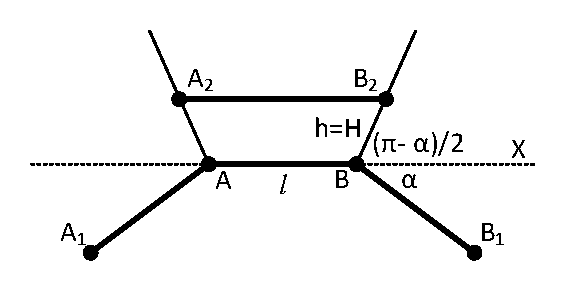
\includegraphics[width=0.6\textwidth]{pics/text_1_remesh_2d/theoretical_rectangles.pdf}
\captionstyle{normal}\caption{Сетка с постоянной кривизной $\alpha$.}
\label{fig:text_1_remesh_2d_theoretical_rectangles}
\end{figure}

Вычислим величину значения $\delta$ для перестроения методом прямоугольников, которая одинаковая для всех ячеек (обозначим ее $\delta_r$).
Для метода прямоугольников имеем $h = H$, $\delta_r = S_{AA_2B_2B} - lH$.
Так как для рассматриваемого примера размер ячейки, кривизна сетки и смещение ячейки постоянно, то $AA_2B_2B$ является трапецией.
Для нахождения площади этой трапеции найдем $\angle B_2BX = \frac{\pi + \alpha}{2} - \alpha = \frac{\pi - \alpha}{2}$.
Тогда имеем следующее выражение для величины $\delta_r$:
\begin{equation}
	\delta_r = \left( l + H \cos \left( \frac{\pi - \alpha}{2} \right) \right) H \sin \left( \frac{\pi - \alpha}{2} \right) - lH
\end{equation}

\begin{figure}[h]
\onelinecaptionstrue
\centering
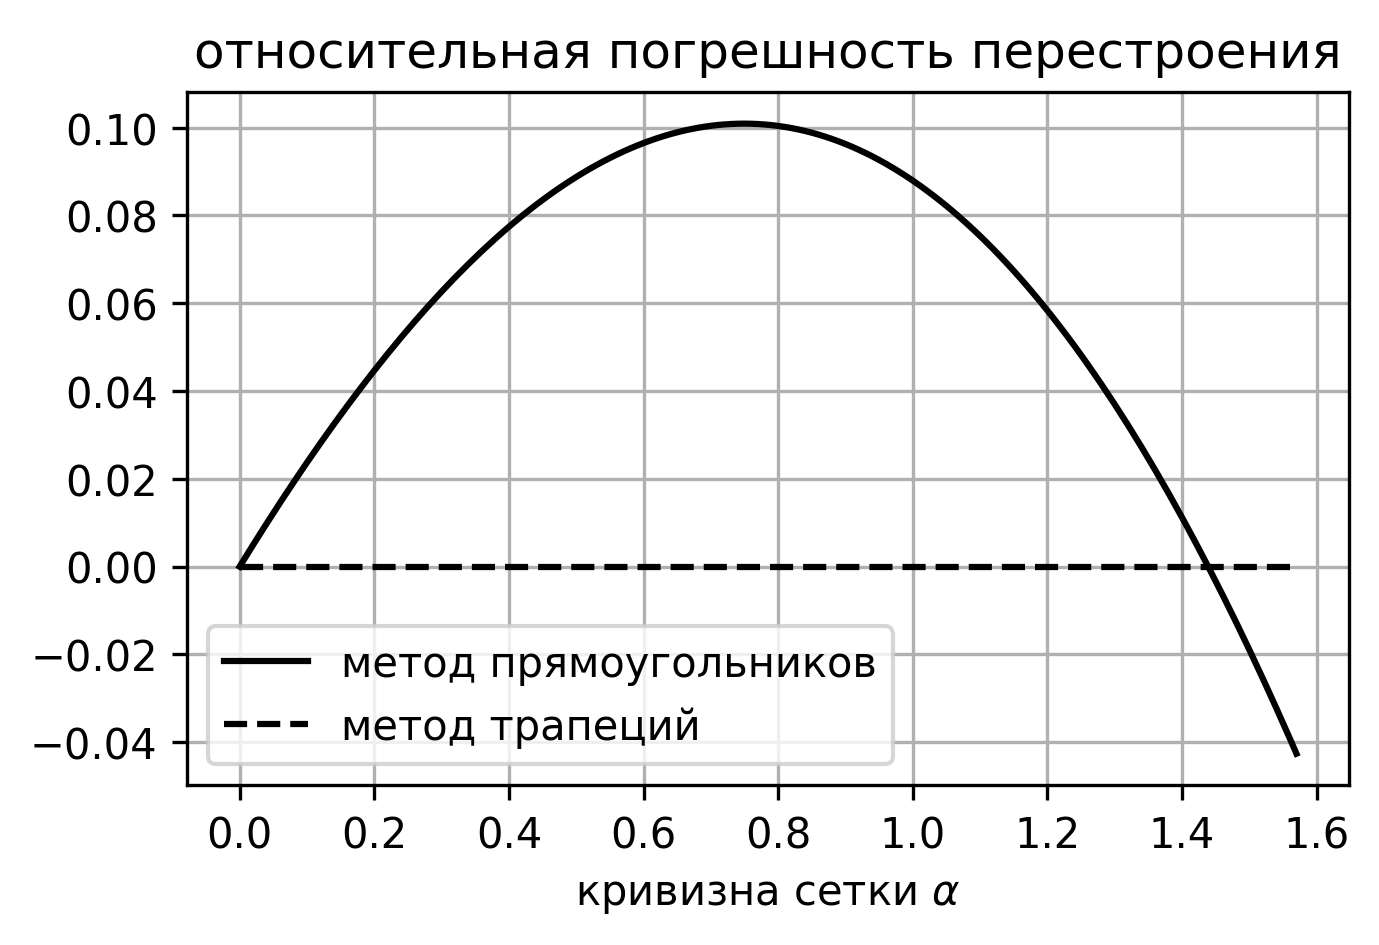
\includegraphics[width=0.7\textwidth]{pics/text_1_remesh_2d/delta_r_lH.png}
\captionstyle{normal}\caption{Теоретическая оценка относительной погрешности перестроения $\frac{\delta_r}{lH}$ для сеток с постоянной кривизной и высотой перестроения.}
\label{fig:text_1_remesh_2d_delta_r_lH}
\end{figure}

Метод трапеций для сеток с постоянными значениями $l$, $H$ и $\alpha$ по своему определению абсолютно точен, то есть в этом случае $\delta_t = 0$.
Результаты теоретических оценок приведены на рис.~\ref{fig:text_1_remesh_2d_delta_r_lH}.

Можно заметить, что результат, полученный на рис.~\ref{fig:text_1_remesh_2d_delta_r_lH} слабо соотносится с результатами практических экспериментов, представленными на рис.~\ref{fig:text_1_remesh_2d_graphic}.
Поэтому требуется анализ точности представленных методов на другой модели перестроения сетки с непостоянным значением $H$.
Рассмотрим такую модель.